%compile with pdflatex on papeeria

\documentclass[a4paper,12pt]{article}
\usepackage{fancyhdr}
\usepackage{fancyheadings}
\usepackage[ngerman,german]{babel}
\usepackage{german}
\usepackage[utf8]{inputenc}
%\usepackage[latin1]{inputenc}
\usepackage[active]{srcltx}
%\usepackage{algorithm}
%\usepackage[noend]{algorithmic}
\usepackage{amsmath}
\usepackage{amssymb}
\usepackage{amsthm}
\usepackage{bbm}
\usepackage{enumerate}
\usepackage{graphicx}
\usepackage{ifthen}
\usepackage{listings}
\usepackage{enumitem}
%\usepackage{struktex}
\usepackage{hyperref}
\usepackage{tikz}
\usepackage{float}
\usepackage{subcaption}
\captionsetup{compatibility=false}
\captionsetup[subfigure]{labelformat=empty}

\usepackage{pgfplots}
\pgfplotsset{compat=1.15}
\usepackage{mathrsfs}
\usetikzlibrary{arrows}

\definecolor{ccqqqq}{rgb}{0.8,0,0}

\pagenumbering{gobble}

%%%%%%%%%%%%%%%%%%%%%%%%%%%%%%%%%%%%%%%%%%%%%%%%%%%%%%
%%%%%%%%%%%%%% EDIT THIS PART %%%%%%%%%%%%%%%%%%%%%%%%
%%%%%%%%%%%%%%%%%%%%%%%%%%%%%%%%%%%%%%%%%%%%%%%%%%%%%%
\newcommand{\Fach}{1. Klausur aus der Mathematik (A)}
\newcommand{\Name}{}
\newcommand{\datum}{}
\newcommand{\Matrikelnummer}{}
\newcommand{\Semester}{Q11/1}
\newcommand{\Uebungsblatt}{} %  <-- UPDATE ME
%%%%%%%%%%%%%%%%%%%%%%%%%%%%%%%%%%%%%%%%%%%%%%%%%%%%%%
%%%%%%%%%%%%%%%%%%%%%%%%%%%%%%%%%%%%%%%%%%%%%%%%%%%%%%

\setlength{\parindent}{0em}
\topmargin -1.0cm
\oddsidemargin 0cm
\evensidemargin 0cm
\setlength{\textheight}{9.2in}
\setlength{\textwidth}{6.0in}

%%%%%%%%%%%%%%%
%% Aufgaben-COMMAND
\newcommand{\Aufgabe}[1]{
  {
  \vspace*{0.5cm}
  \textsf{\textbf{Aufgabe #1}}
  \vspace*{0.2cm}
  
  }
}
%%%%%%%%%%%%%%
\hypersetup{
    pdftitle={\Fach{}: Übungsblatt \Uebungsblatt{}},
    pdfauthor={\Name},
    pdfborder={0 0 0}
}

\lstset{ %
language=java,
basicstyle=\footnotesize\tt,
showtabs=false,
tabsize=2,
captionpos=b,
breaklines=true,
extendedchars=true,
showstringspaces=false,
flexiblecolumns=true,
}

\title{Übungsblatt \Uebungsblatt{}}
\author{\Name{}}

\begin{document}
\thispagestyle{fancy}
%\lhead{\sf \large \Fach{} \\ %\small \Name{} - \Matrikelnummer{}
\lhead{\sf \large \Fach{} %\small \Name{} - \Matrikelnummer{}
}
\rhead{\sf \Semester{}   \datum{}}
%\rhead{\sf \Semester{} }
\vspace*{0.2cm}
%\begin{center}
%%\LARGE \sf \textbf{Übungsblatt \Uebungsblatt{}}
%\end{center}
%\vspace*{0.2cm}

%%%%%%%%%%%%%%%%%%%%%%%%%%%%%%%%%%%%%%%%%%%%%%%%%%%%%%
%% Insert your solutions here %%%%%%%%%%%%%%%%%%%%%%%%
%%%%%%%%%%%%%%%%%%%%%%%%%%%%%%%%%%%%%%%%%%%%%%%%%%%%%%

  Name: \underline{\hspace{7cm}}
  \hfill
  Datum: \underline{\hspace{4cm}}

%\vspace{0,5cm}Die Rechenwege müssen nachvollziehbar sein!
%
%\vspace{0,5cm} {TEIL A} - ohne Hilfsmittel - Bearbeitungszeit 30 Minuten
\vspace {2cm}
% 
%GEOMETRIE

\Aufgabe{1:}
Entscheiden Sie, ob die folgenden Aussagen wahr oder falsch sind. Begründen Sie jeweils in einem Satz die falschen Aussagen. (Achtung: für fehlende oder falsche Angaben werden Punkte abgezogen!)\\

Gegeben ist die Funktion 
\[f: x \rightarrow \frac{3x-6}{(x+3)^2(x-2)}\]

\begin{enumerate}[label={\alph*)}]
  \item Die Definitionsmenge von $f$ ist $D_f = \{-3; 2\}$.
  \item Der Graph $G_f$ schneidet die $y$-Achse oberhalb des Ursprungs.
  \item Der Graph $G_f$ hat ein Loch.
  \item Die Funktion $f$ hat einen Pol mit Vorzeichenwechsel.
  \item Der Punkt $P(-1|2,25)$ liegt auf $G_f$.
  \item Die Wertemenge ist $W_f = ]0; \infty[$.
\end{enumerate}


\Aufgabe{2:}
Gegeben ist die Funktion $f$ mit
\[ f(x) = \frac{x^2+1}{(x+1)^2} \]
\begin{enumerate}[label={\alph*)}]
  \item Bestimmen Sie die Definitionsmenge und die Schnittpunkte mit den Koordinatenachsen.
  \item Ermitteln Sie das Verhalten an den Grenzen des Definitionsbereichs.\\
    Geben Sie die Gleichungen aller Asymptoten an.
  \item Bestimmen Sie Art und Lage des Extrempunkts von $G_f$.
  \item Bestimmen Sie Krümmungsverhalten und Lage des Wendepunkts von $G_f$.
  \item Skizzieren Sie unter Verwendung aller bisherigen Ergebnisse den Graphen von $f$.
\end{enumerate}


\Aufgabe{3:}
\begin{enumerate}[label={\alph*)}]
  \item Gegeben ist die Funktion $f$ mit 
    \[ f(x) = x^2+3x-1 \]\\
    Ermitteln Sie mit Hilfe des Differentialquotienten die Ableitung der Funktion $f(x)$.
    \item Skizzieren Sie zum gegebenen Graph der Funktion $h$ die zugehörige Ableitungsfunktion $h'$ (direkt im gegebenen Koordinatensystem)

\begin{figure}[h!]
  \begin{center}
    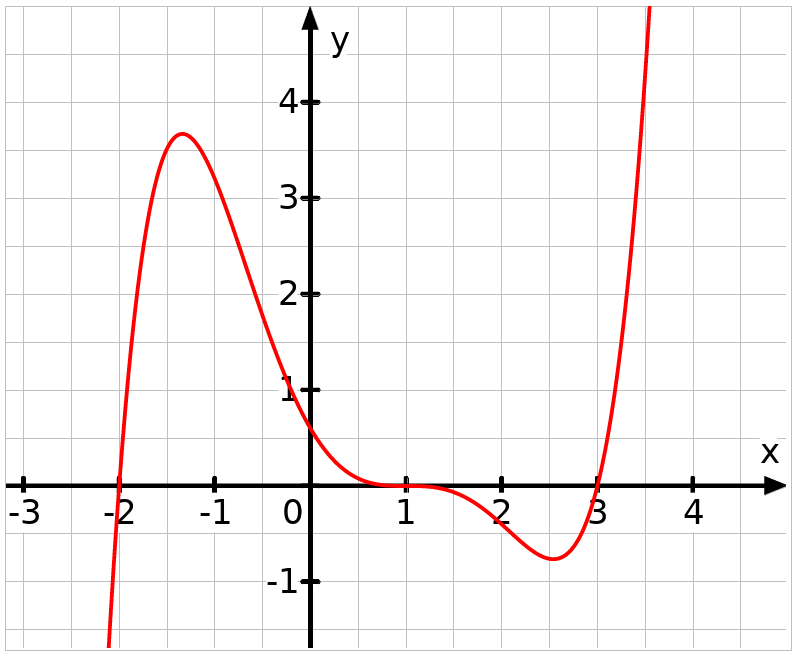
\includegraphics[width=0.9 \linewidth]{Q11_1KlausurJanuar2022_1.png}
  \end{center}
\end{figure}

\end{enumerate}

\newpage
\enlargethispage{4cm}
\Aufgabe{4:}
Gegeben ist die Funktion 
\[f:x \rightarrow \frac{x^2-a}{x^2-b} \quad \text{mit $a\neq b$}\]

\begin{enumerate}[label={\alph*)}]
  \item Geben Sie einen Wert für $b$ an, so dass die Funktion $f$ für alle reellen Zahlen definiert ist.
  \item Bestimmen Sie die Nullstellen von $f$ in Abhängigkeit von $a$. (Fallunterscheidung!)
  \item Einer der drei abgebildeten Graphen gehört zum Fall $0 < a < b$.\\
    Geben Sie an, welcher dies ist, und begründen Sie Ihre Antwort, indem Sie erläutern, warum die beiden anderen Fälle ausscheiden.
\end{enumerate}

\begin{figure}[h!]
  \begin{center}
    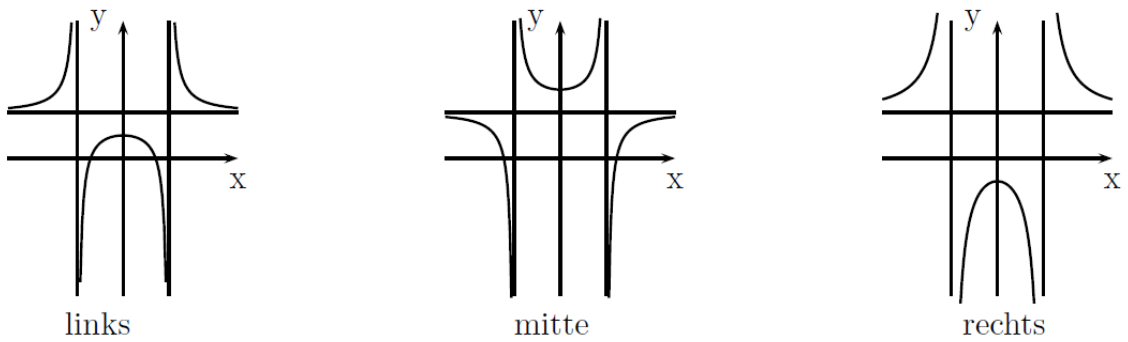
\includegraphics[width=0.7 \linewidth]{Q11_1KlausurJanuar2022_2.png}
  \end{center}
\end{figure}


\Aufgabe{5:}

\noindent
\begin{minipage}{0.6\textwidth}%\raggedleft
Bei einem Rennen 1999 in Silverstone versagten bei Michael Schumacher Bremsen und Lenkung vor Einfahrt in die Stowe-Kurve. Der Streckenverlauf wird durch den Graph der Funktion $f$ mit
\[f(x)=-\frac{1}{3}x^2+3 \]
angenähert, sein Wagen verlässt die Fahrbahn an der Stelle $x_0 = -3$.
\end{minipage}
\hfill%
\begin{minipage}{0.3\textwidth}% adapt widths of minipages to your needs
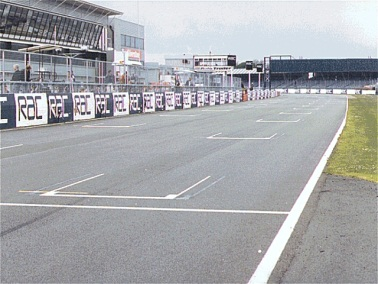
\includegraphics[width=\linewidth]{Q11_1KlausurJanuar2022_3.png}
\end{minipage}%


%\begin{figure}[h!]
%  \begin{center}
%    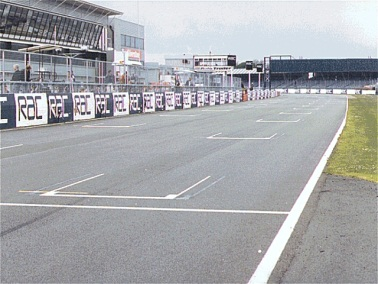
\includegraphics[width=0.4 \linewidth]{Q11_1KlausurJanuar2022_3.png}
%  \end{center}
%\end{figure}

\begin{enumerate}[label={\alph*)}]
  \item Bestimmen Sie die Gleichung der Funktion, die den weiteren Fahrtverlauf nach dem Versagen der Bremsen und der Lenkung beschreibt.\\
    \\
    Im Punkt $A(3|12)$ trifft der Ferrari auf die aufgestapelten Autoreifen, die den Aufprall auf die Mauer dämpfen sollen. Beim Aufprall fliegt das linke Vorderrad im rechten Winkel zur Aufprallrichtung davon.
  \item Bestimmen Sie die Gleichung der Funktion, die die Flugbahn des Reifens beschreibt.
\end{enumerate}



\centerline{Viel Erfolg}
%\enlargethispage{2\baselineskip}

%\addtolength{\voffset}{-2cm}




%\begin{tikzpicture}
%\draw [very thin, black, step=0.5cm] (0,0) grid +(15,18);
%\end{tikzpicture}


\newpage
\Aufgabe{1: Musterlösung}
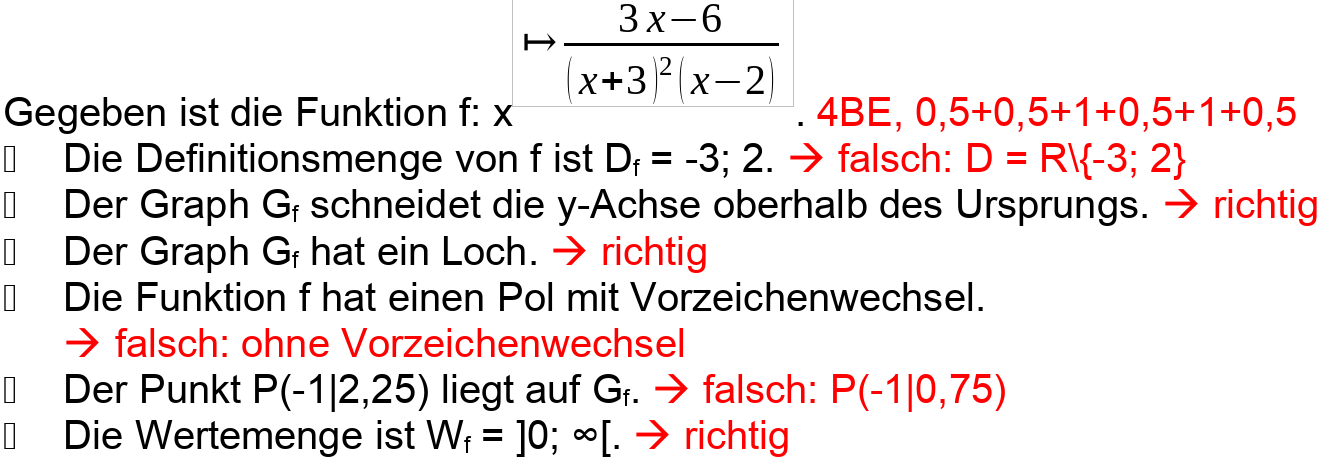
\includegraphics[width=\linewidth]{Q11_1KlausurJanuar2022_ml1.png}

\Aufgabe{2: Musterlösung}
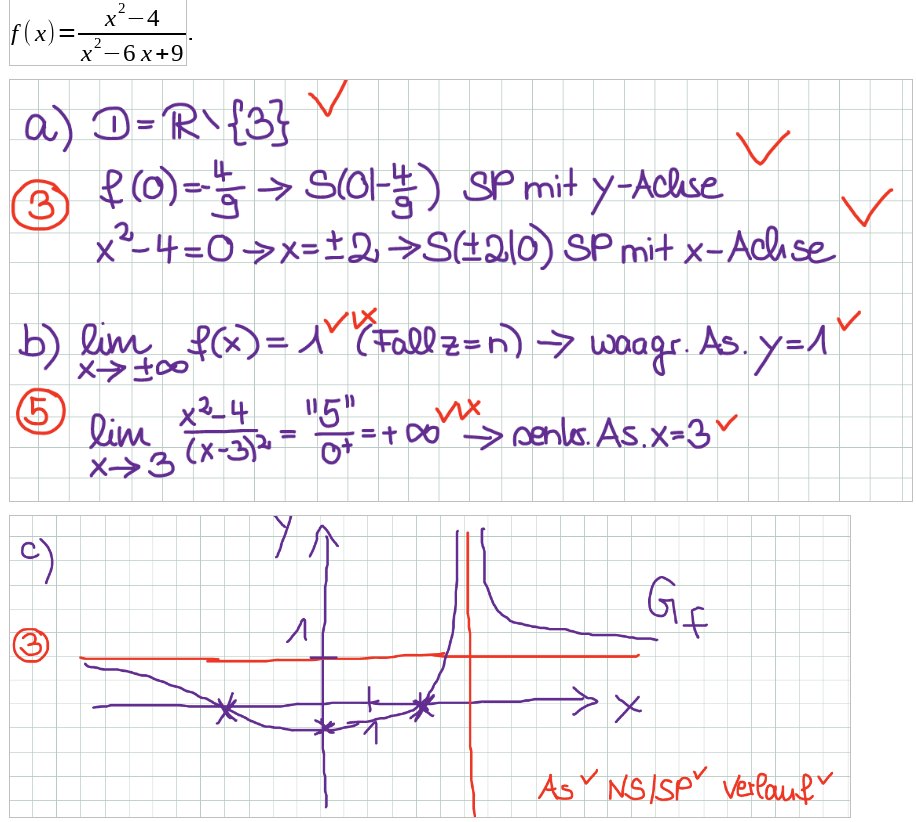
\includegraphics[width=\linewidth]{Q11_1KlausurJanuar2022_ml2.png}

\newpage
\Aufgabe{3: Musterlösung}
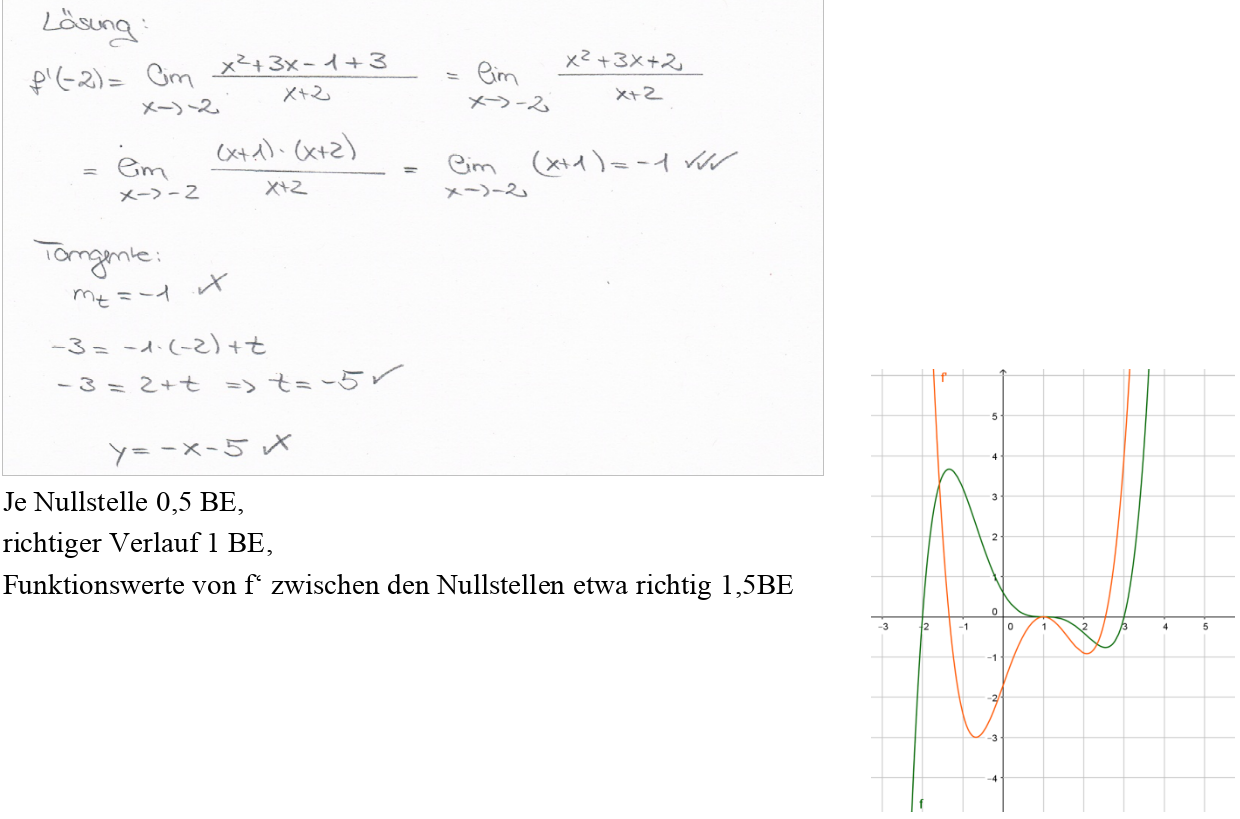
\includegraphics[width=\linewidth]{Q11_1KlausurJanuar2022_ml3.png}

\Aufgabe{4: Musterlösung}
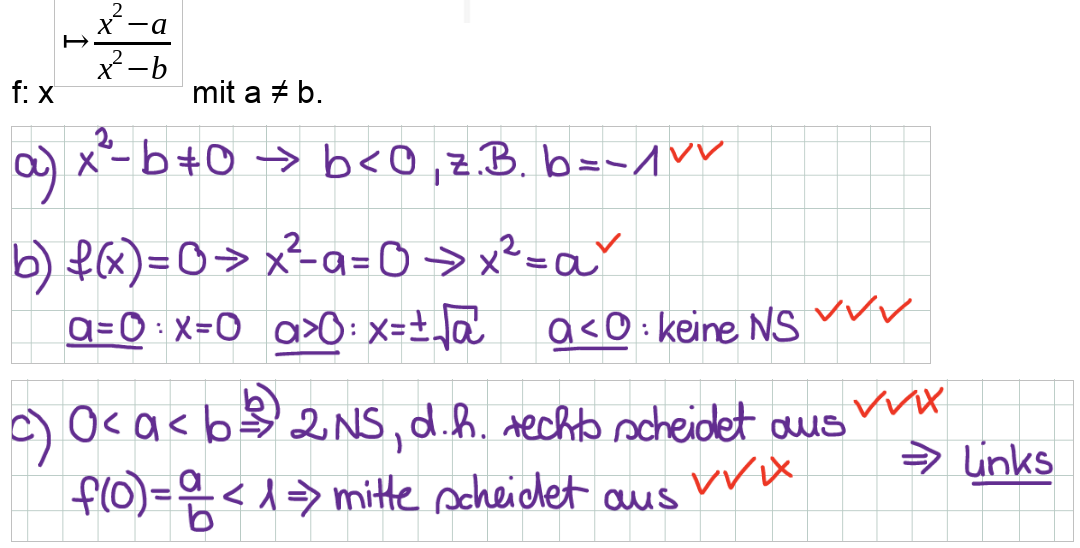
\includegraphics[width=\linewidth]{Q11_1KlausurJanuar2022_ml4.png}

\newpage
\Aufgabe{5: Musterlösung}
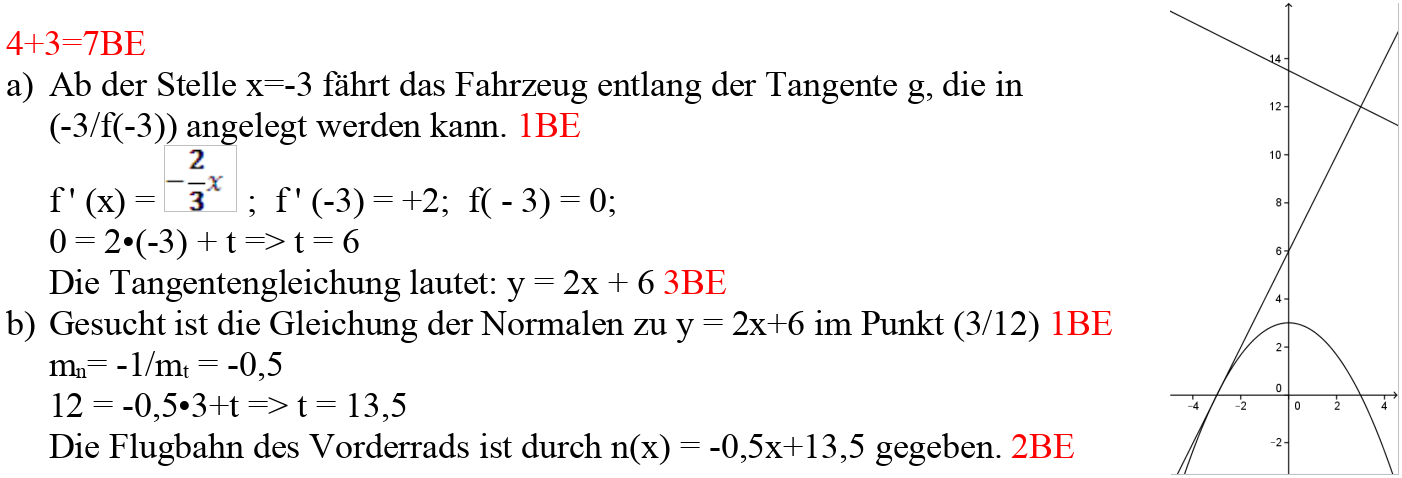
\includegraphics[width=\linewidth]{Q11_1KlausurJanuar2022_ml5.png}


%%%%%%%%%%%%%%%%%%%%%%%%%%%%%%%%%%%%%%%%%%%%%%%%%%%%%%
%%%%%%%%%%%%%%%%%%%%%%%%%%%%%%%%%%%%%%%%%%%%%%%%%%%%%%
\end{document}
